\documentclass{standalone}
\usepackage{tikz}


\begin{document}

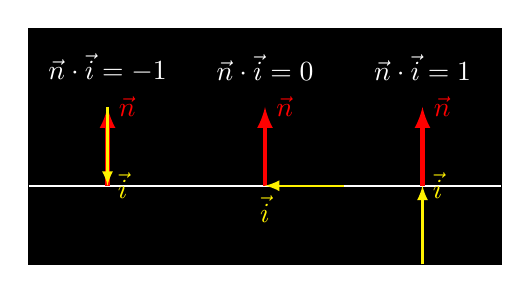
\begin{tikzpicture}
  \draw[fill=black,black] (-1,-1) rectangle (5,2);

  \begin{scope}
    \draw[thick,white] (-1,0) -- (1,0);
    \draw[ultra thick,red,-latex] (0,0) -- (0,1) node[right] {$\vec n$};
    \draw[thick,yellow,-latex] (0,1) -- (0,0) node[right] {$\vec i$};
    \node[white] at (0,1.5) {$\vec n \cdot \vec i = -1$};
  \end{scope}

  \begin{scope}[xshift=2cm]
    \draw[thick,white] (-1,0) -- (1,0);
    \draw[ultra thick,red,-latex] (0,0) -- (0,1) node[right] {$\vec n$};
    \draw[thick,yellow,-latex] (1,0) -- (0,0) node[below] {$\vec i$};
    \node[white] at (0,1.5) {$\vec n \cdot \vec i = 0$};
  \end{scope}


  \begin{scope}[xshift=4cm]
    \draw[thick,white] (-1,0) -- (1,0);
    \draw[ultra thick,red,-latex] (0,0) -- (0,1) node[right] {$\vec n$};
    \draw[thick,yellow,-latex] (0,-1) -- (0,0) node[right] {$\vec i$};
    \node[white] at (0,1.5) {$\vec n \cdot \vec i = 1$};
  \end{scope}
\end{tikzpicture}

\end{document}